\chapter{序論}
\label{chapter:introduction}

本章では,本研究の実施に至った背景を説明し,対象とする課題を明確にする.

%------------------------------------------------------------------------
\section{本研究の背景}
  \subsection{街中における看板}
  \label{subsection:signboards_in_town}
    現在,都市には多種多様な視覚情報が溢れている.
    都市に多く存在する視覚情報の1つとして,屋外広告物である看板が挙げられる.
    看板の目的は,看板を掲示する場所に存在する店舗や会社の名称の掲示が主である.
    店舗は不特定多数の人々に対して来店を訴求するために看板を掲示し,人々は目に入った看板に描かれているデザインや文字から何らかの影響を受けて,具体的な行動に移す\cite{Koyama:2016}.
    例えば,人々が都市空間において店舗を探す際,看板に描かれている内容から,飲食店や衣料販売店などの店舗の種類を判別し,どの店に入るかなどの意思決定を行っている.
    しかし,繁華街など店舗が多数存在する地域においては,都市環境への配慮が十分でなく,「目立つこと」「インパクトがあること」「興味を引くこと」が優先され,看板やネオンによって埋め尽くされた景観が形成されている場合がある\cite{Yokokawa:2000}.
    このような場合においては,看板がひしめき合うことで,逆に視覚情報が見えにくくなるという現象を引き起こしている\cite{Watanabe:2003}.
    そのため,看板が街を行き交う歩行者に対して情報を与えるという本来の役割を果たせていないという問題がある.

    また,看板から得られる情報は限定的である.
    看板から店舗の種類などの基本的な情報は取得できるが,その店舗で享受できるサービスの詳細な内容まで取得することはできない.
    そのため,見慣れない看板からその店舗の詳細情報を得ることは容易ではない.

  \subsection{看板情報の多言語性}
    近年,日本を訪れる観光客は増加しつつある.
    日本政府観光局によると,2012年に8,358,105人であった訪日観光客は,2017年には28,691,073人と,3倍を超えて増加している\cite{JNTO:2018}.
    こうした訪日外国人の増加にも関わらず,店舗の看板などは多言語で記載されているとは限らない.
    看板情報の多くは地元の言語で書かれており,それが言語障壁を引き起こしている.
    例えば,日本語が理解できるユーザは,図\ref{figure:kabukicho}のような地域においては,目の前の店舗がどのような店舗なのかを理解できることが多い.
    しかし,図\ref{figure:myeongdong}のような地域では,韓国語の文字が読めなければ,目の前にある店舗の種類や享受できるサービスなどの情報を看板から得ることは困難である.

    さらに,外国人にとっては,看板に書かれている文字が母国語に翻訳されたとしても,それによって内容を理解できるとは限らない.
    林田らは,日本に不慣れな外国人が,街の中でどのような情報を必要としているのかを調査するために,日本人と外国人それぞれに情報要求調査実験を行った\cite{Hayashida:2005}.
    その結果,日本人からはあまり出なかった要求情報として,例えば「これが竹林ですか?」のような,自身の持っている知識と現在見ているものとの関連を尋ねるようなものがあった.
    日本人であれば,「これがあの有名な五条橋?」と考えることはあっても,五条橋と書いてあったり,観光客が多かったり,常識を使って考えることで判断できる場合が多い.しかし,外国の人にとっては新鮮でも,日本人にとっては常識であるものが対象であると,「これが竹林です」という立看板は中々作られない為,受動的に取得できる情報だけでは,知識との照会がスムーズにできない.
    店舗の看板を例に挙げると,日本語の看板に店舗名がローマ字で併記されていたとしても,日本語が分からなければ,それが店の名前であることが分からない.
    このように,外国人観光客は日本人の多くが常識として持っている情報を持っていないことも多く,外国人にとってはどの店がどのようなサービスを行っているか,クレジットカードでの決済はできるかなどの情報を看板から得ることは容易ではない.
    このように,日本人に与えられている情報をただ翻訳して伝えるだけでは不十分である.

\section{街中における検索行為}
\label{section:searching_action}
  人々が街中において求める条件に合致した店舗を探す際に用いる情報には,主に(1)店舗の看板や外観から取得した情報,(2)ガイドブックやガイドマップに掲載されている情報,(3)スマートフォン等の携帯端末で検索して得た情報,が挙げられる.
  例えば,人々が飲食店を探す場合,飲食店の看板や案内はユーザにとって必要な情報であり,それ以外の衣料店などの情報は不要な情報に分類できる.

  (1)を用いる場合は,全国展開しているチェーン店などのユーザが見慣れた店舗である場合,情報は容易に取得できるが,ユーザが知らない店舗である場合,看板に書かれている店舗名や外観からのみでは店舗の詳細情報が十分に得られない可能性がある.そのため,「低価格の和食の店」などのユーザが求める条件に合う店舗なのかを素早く知る手法が求められる.

  (2)を用いる場合は,選択肢がガイドブックやガイドマップに掲載されている店舗に限られてしまうという制約があるが,その中からユーザが求める条件に合致する店舗を発見し,それに掲載されている情報から,店舗の詳細情報を容易に得ることはできる.しかし,ユーザが慣れていない地域において,ガイドブック等に記載されている地図を頼りに店舗を探し出すことは容易ではない.

  (3)を用いる場合は,現状ではスマートフォンなどの携帯端末を用いて,位置情報を手がかりに周辺の検索を行うことで,求める条件に合致した店舗情報を探している.
  Google Map\footnote{\url{https://www.google.com/maps}(2019/1/14存在確認)}などの地理情報システムには,住所から地図上の位置を特定する機能があり,飲食店に限定すると,食べログ\footnote{\url{https://tabelog.com}(2019/2/6存在確認)}やyelp\footnote{\url{https://www.yelp.com}(2019/2/6存在確認)},OpenTable\footnote{\url{https://www.opentable.co.uk}(2019/2/6存在確認)}などのWebサービスが数多く展開されている.このようなWebサービスには,店舗側が自身の店舗の営業時間や価格などの詳細情報を登録したり,ユーザが店舗のレビューを投稿したりでき,現在地周辺のレストランを検索する機能や,ユーザによるレストランの評価を確認する機能などを持っている.
  しかし,位置情報を用いるのみではユーザが実際に見ている看板や標識などの現実世界上における正確な位置まで提示できず,ユーザがいる環境と検索行為とが分断されており,その環境から目的の店舗を探す手間が残されている.
  
  このように,現実世界において店舗を探索する際,看板はその店で享受できるサービスの種類を知る上で重要な役割を果たしているが,図\ref{figure:kabukicho}や図\ref{figure:myeongdong}のように看板が密集している地域においては,一軒一軒の店舗情報を検索する必要があり,目的とする情報の探索に少なからず時間を要してしまう.
  そのため,探索する看板が未知であるものや,目立たないものである場合,大量に存在する他の視覚情報に紛れて見つけることができない可能性があり,目的の店舗を発見することは容易ではない.
  特に,初めて訪れる場所など,慣れていない地域でユーザが看板などの視覚情報を探す場合,特定の情報を素早く見つけることは容易ではないという問題がある.

  ユーザがその地域の言語を理解でき,言語障壁がない場合は時間を掛けることで条件に合致する店舗を探せるが,ユーザが外国人観光客の場合,自身の目の前にある店舗が自身の求める条件に合致するかスマートフォンで検索しようとしても,言語障壁によりどのように検索して良いか分からない場合がある.
  さらに,位置情報を用いて周辺の店舗情報を検索し,条件に合う店舗が見つかったとしても,その店舗の看板に書かれている文字を読むことができなければ,多数ある店舗の中から目的の店舗を発見することは容易ではない.
  そのため,結局ガイドマップに記載されている店舗など,限られた選択肢から選択せざるを得ない状況にある.
  店舗側が看板を多言語化することや,QRコードなどを用いて多言語で情報を配信する手法を採ることでこの問題は解決できる可能性があるが,様々な言語圏からの来訪者すべてに対応するには限界があり,このような手法では店舗側の負担も大きいという問題がある.

\section{本研究の目的}
\label{section:purpose}
  \ref{section:searching_action}節で述べた問題を解決するために,本研究では,繁華街や商店街などユーザの周囲に店舗が多数存在する地域を,携帯端末のカメラを通して見た際に,
  (1)視覚情報の識別性を向上させ,ユーザが目的の店舗を見つけるのに要する時間を短縮させること,
  (2)ユーザが慣れていない地域や周囲の文字が読めない状況であっても,目の前にある店舗の情報を直感的かつ簡単に取得できるようにすること,の2点を目的とする.

  (1)を実現するために,先行研究\cite{Fujita:2013}で提案されたユーザにとって不要な情報を目立たなくさせる手法を改良し,必要な情報に付加情報を重畳表示する提示手法を提案する.さらに,全天球カメラで撮影した画像内において,条件に合う店舗を探索するプロトタイプを実装する.これにより,視覚情報が密集している地域において,ユーザが迷うことなく目的の店舗を発見できるようになることが期待される.

  (2)を実現するために,スマートフォンを店舗の看板にかざすことで,地理情報システムのデータベースに登録されている店舗情報を取得し,カメラ映像上に店舗情報を重畳表示するシステムを提案する.
  大河原らによると,店舗情報を円形ツリーマップ等を用いて視覚化することによって,店舗の全体像の把握が容易になり,素早く店舗を回遊できることが明らかとなっている\cite{Ookawara:2015}.
  看板の認識には多くの画像データが必要であるため,特定の地域を対象とした実環境で利用できるプロトタイプを実装する.これにより,言語障壁があっても,ユーザが目の前の店舗でどのようなサービスが得られるのかを知ることができるようになり,求める条件に合致した店舗を直感的に選択できるようになることが期待される.

  本稿ではこれらの提案システムの優位性を検証するために従来手法と比較したユーザ実験を行い,その結果について述べる.

  \begin{figure}[tb]
    \centerline{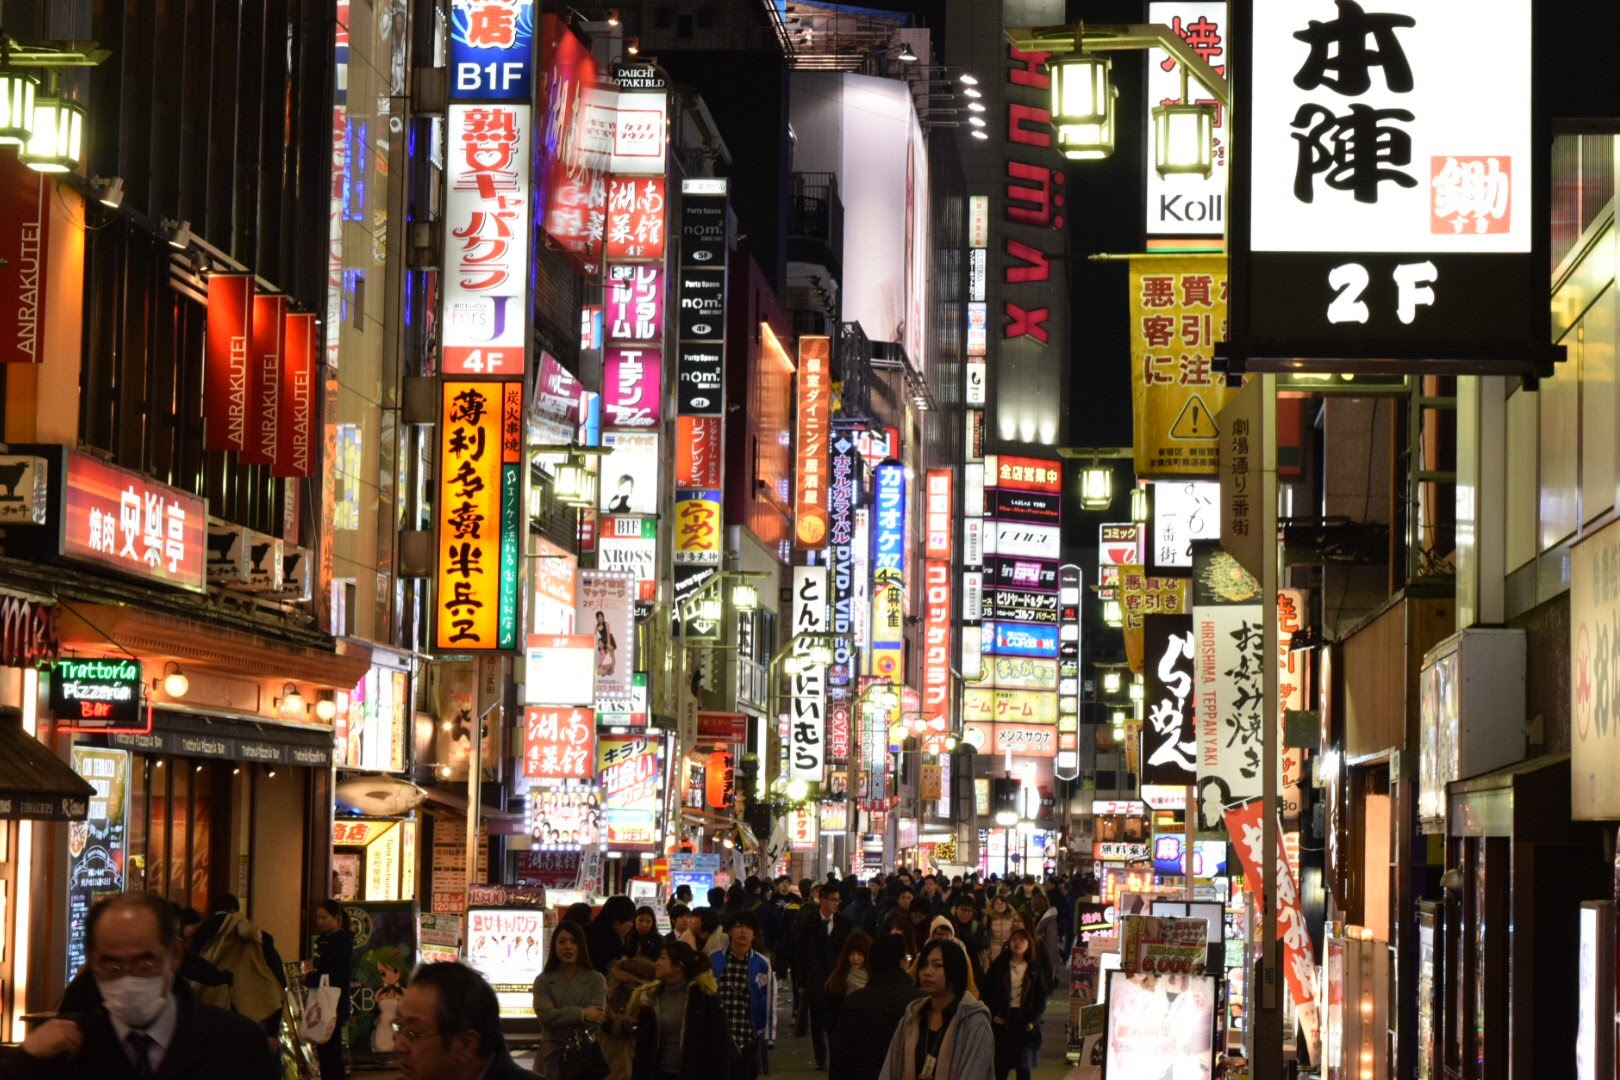
\includegraphics[width=.9\columnwidth, clip]{kabukicho.jpg}}
    \caption{密集する看板情報(新宿・歌舞伎町)}
    \label{figure:kabukicho}
    \vspace{1cm}
    \centerline{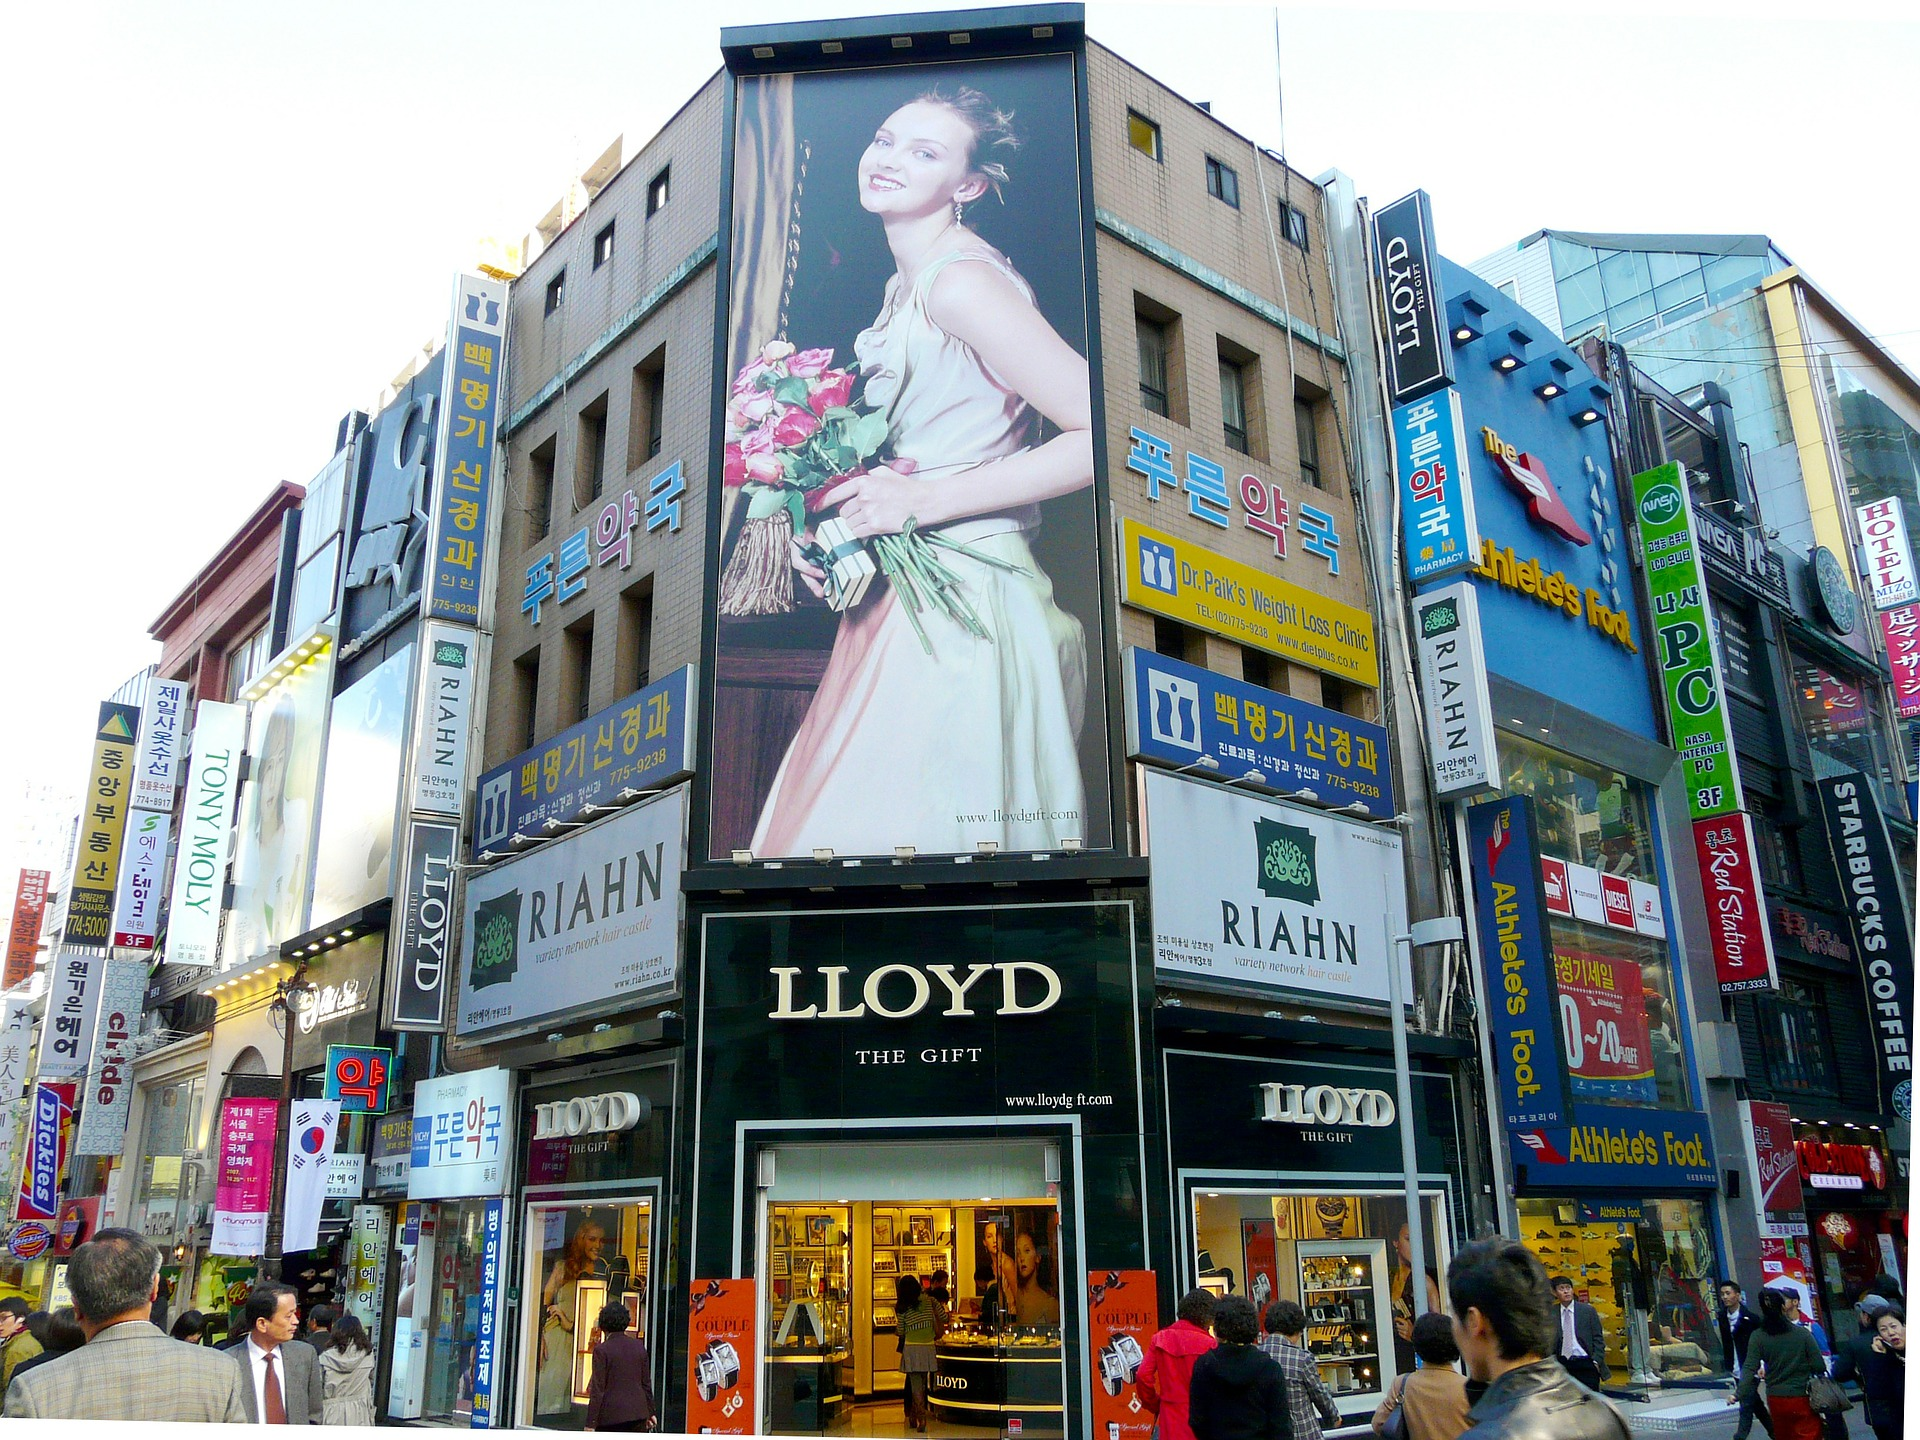
\includegraphics[width=.9\columnwidth, clip]{myeongdong.jpg}}
    \caption{密集する看板情報(韓国・明洞)}
    \label{figure:myeongdong}
  \end{figure}
